\documentclass[a4paper]{article}
\usepackage[fontset=fandol]{ctex}
\usepackage[margin=1.65cm]{geometry}
\usepackage{amsmath,amssymb}
\usepackage{graphicx}
\usepackage{hyperref}
\usepackage{longtable,booktabs}
\usepackage{xcolor}
\usepackage{enumitem}
\usepackage{listings}
\lstset{basicstyle=\ttfamily\small,breaklines=true,columns=fullflexible,keepspaces=true}
\hypersetup{colorlinks=true,linkcolor=blue,urlcolor=blue}
\setlist[itemize]{leftmargin=1.25em,itemsep=0.18em}
\setlength{\parskip}{0.45em}
\setlength{\parindent}{2em}
\sloppy
\title{第 03 讲：现代 Transformer architecture 与 hyperparameters}
\author{CS336 Spring 2026 public videos and official course materials}
\date{}
\begin{document}
\maketitle
\tableofcontents
\newpage
\section{本章导读}
本章讨论 \textbf{现代 Transformer architecture 与 hyperparameters}。CS336 的第一层目标不是把现成大模型当作黑箱使用，而是把 language model 从输入文本、训练目标、模型结构、数据、系统和评估这些部件重新拆开。只有拆开之后，读者才能判断一个设计选择究竟改变了什么。
设想你要从论文表格里选择一个 decoder-only Transformer recipe。所有候选模型都叫 Transformer，但 pre-norm、RMSNorm、RoPE、SwiGLU、QK norm、head layout 和 learning rate schedule 不同；本章训练你判断哪些是核心机制，哪些是经验性工程选择。
本章对应 CS336 Spring 2026 第 03 个公开视频，并结合课程页提供的可解析资料。视频和课程页给出事实边界；正文把这些材料改写为可自学的教材章节。
阅读本章时，先理解问题为什么存在，再看定义、公式和实现形态，随后通过例题和练习检查自己是否能独立复现这条 reasoning chain。
\begin{figure}[h]
\centering

\includegraphics[width=0.58\linewidth]{source_anchor.jpg}
\caption{第 03 讲的课程图像锚点。}
\end{figure}
\subsection{本章知识路线}
\begin{itemize}
\item 本章首先说明 现代 Transformer architecture 与 hyperparameters 为什么是 language modeling pipeline 中不可跳过的一环。
\item 其次定义本章反复使用的术语，并说明这些术语对应的计算对象或系统对象。
\item 随后用公式和伪代码表达主要机制，让概念能够落到可计算的变量上。
\item 最后给出例题、风险讨论和练习，便于读者检查自己是否真正掌握了机制。
\end{itemize}
\subsection{结构图}
下面的图用于帮助读者定位本章的核心结构。先看概念之间的依赖，再回到正文中的公式、伪代码和例题。
\begin{figure}[h]
\centering
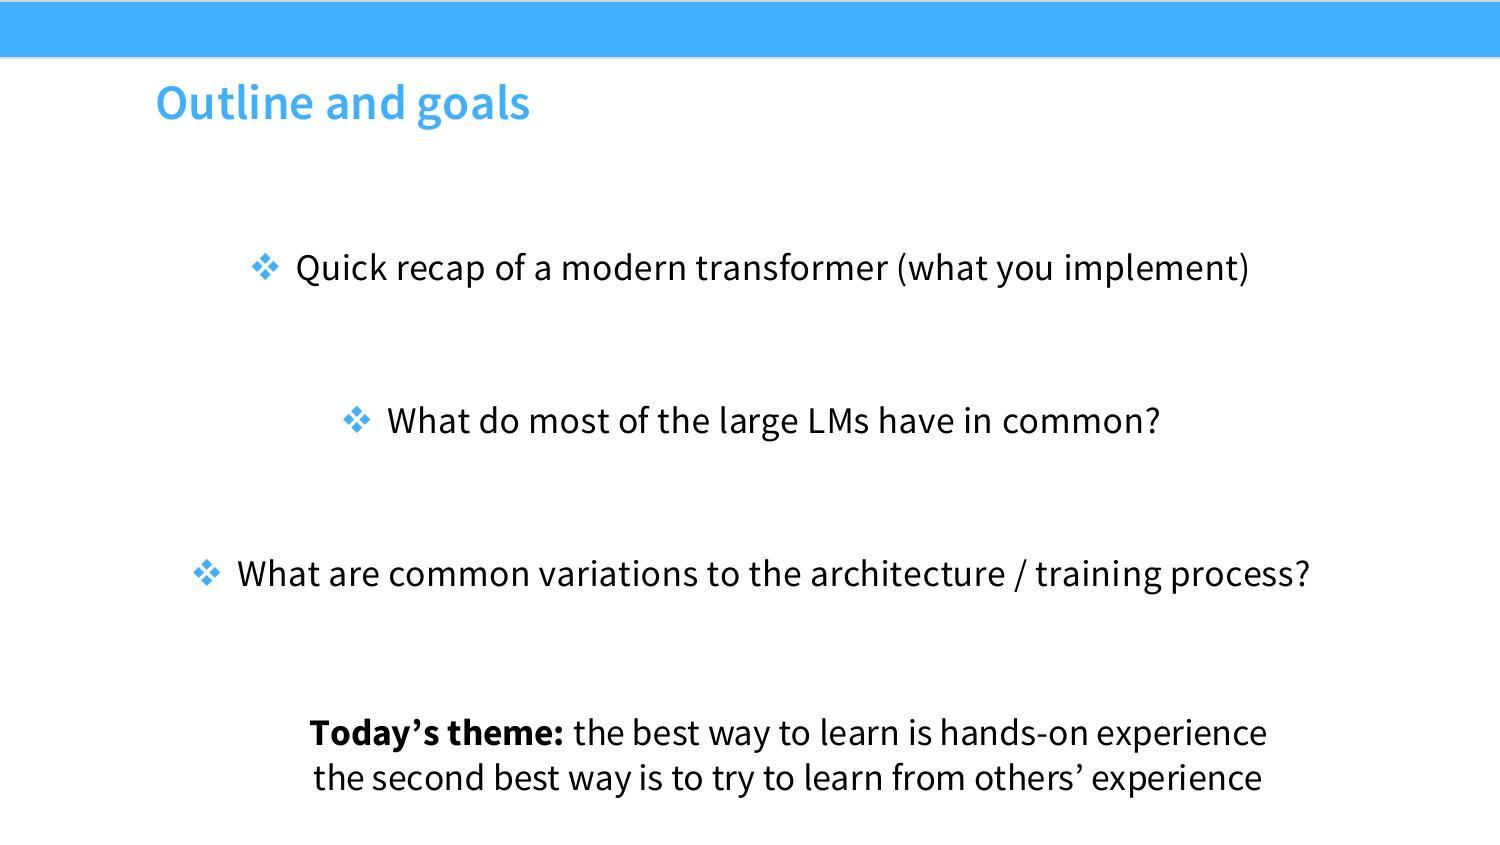
\includegraphics[width=0.72\linewidth]{pdf_pages/page-02.jpg}
\caption{官方材料图页：现代 Transformer architecture 与 hyperparameters 的课程页/PDF/script 图像锚点。}
\end{figure}
\begin{figure}[h]
\centering
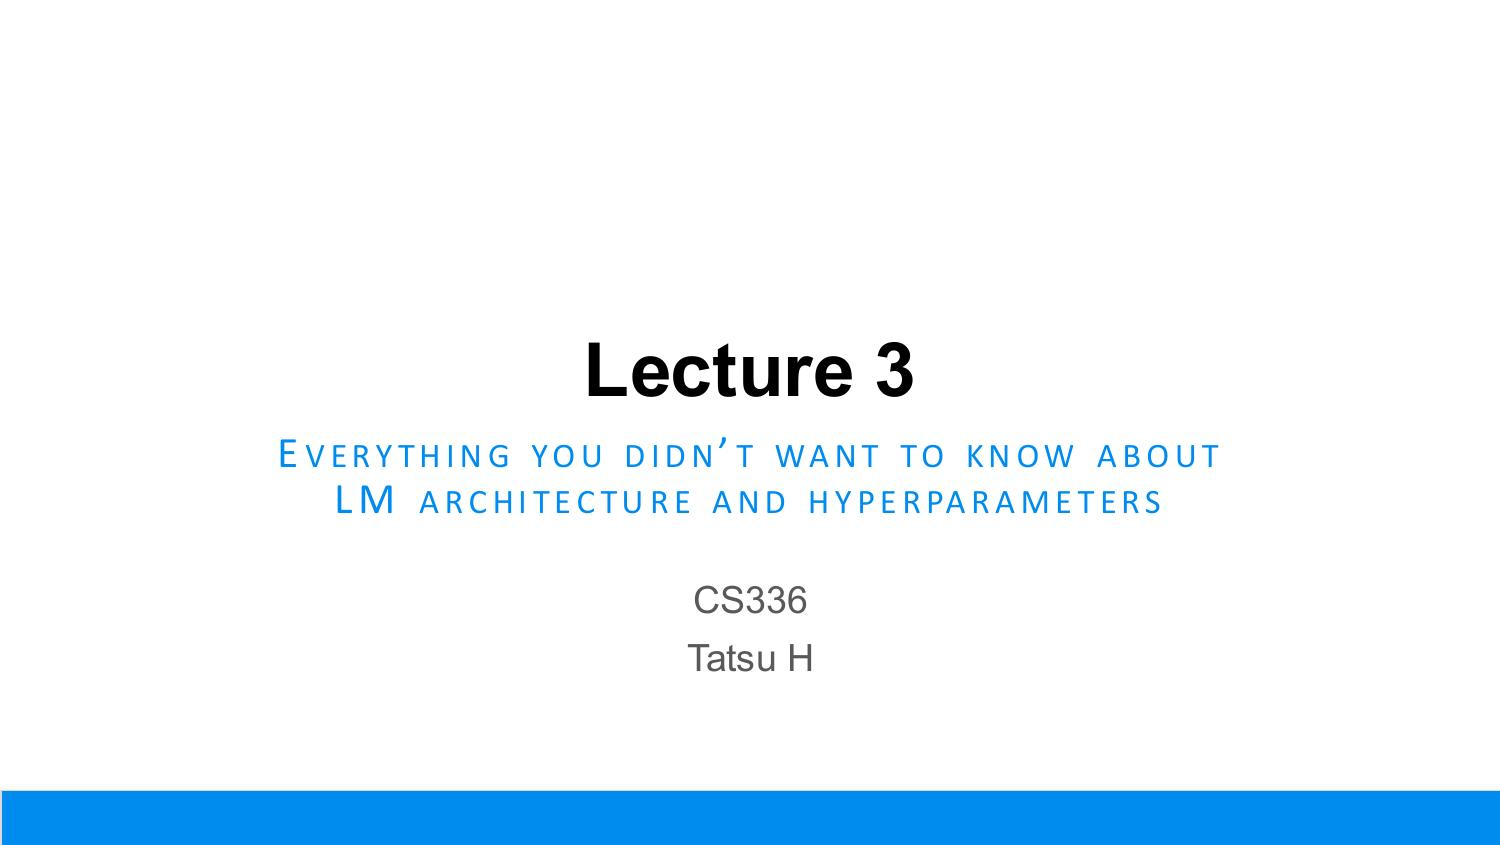
\includegraphics[width=0.72\linewidth]{pdf_pages/page-01.jpg}
\caption{官方材料图页：现代 Transformer architecture 与 hyperparameters 的课程页/PDF/script 图像锚点。}
\end{figure}
\section{本章主线}
本章可以沿着三条线索阅读：课程为什么把这个主题放在这里，它改变了哪些变量，以及怎样用小实验检查这些变量。
\subsection{本章要解决的核心问题}
本讲从现代 decoder-only Transformer 的共同骨架出发，比较 LLaMA-like 架构里的 pre-norm、RMSNorm、RoPE、SwiGLU、bias removal、QK norm 等设计。
这一点对应的学习动作是：找出对象，写出变量，说明变量如何被测量。若输入规模、硬件、数据分布或评估协议改变，结论也必须重新检查。
因此，现代 Transformer architecture 与 hyperparameters 不应被读成若干名词的集合，而应被读成一组可检验的机制。
\subsection{从机制到资源账本}
架构选择不能脱离 scale。小模型 ablation 中看似微弱的差异，在大模型训练中可能表现为稳定性、吞吐、长上下文或超参数敏感性的差异。
这一点对应的学习动作是：找出对象，写出变量，说明变量如何被测量。若输入规模、硬件、数据分布或评估协议改变，结论也必须重新检查。
因此，现代 Transformer architecture 与 hyperparameters 不应被读成若干名词的集合，而应被读成一组可检验的机制。
\subsection{从课堂讲解到可复现实验}
hyperparameter 的有效读法是把每个选择对应到 failure mode：学习率过大导致发散，batch 太小导致噪声过大，context 太长带来 attention 和 KV cache 成本，width/depth 比例影响计算形状。
这一点对应的学习动作是：找出对象，写出变量，说明变量如何被测量。若输入规模、硬件、数据分布或评估协议改变，结论也必须重新检查。
因此，现代 Transformer architecture 与 hyperparameters 不应被读成若干名词的集合，而应被读成一组可检验的机制。
\section{术语、符号与问题边界}
本章的术语横跨模型、数据和系统。读者需要先知道每个词指向的对象：有些词描述数学目标，有些词描述张量形状，有些词描述硬件瓶颈，还有一些词描述评估协议。术语边界不清，后面的公式和实现就会变成空洞的缩写。
\begin{longtable}{p{0.08\linewidth}p{0.42\linewidth}p{0.42\linewidth}}
\toprule
\textbf{\#} & \textbf{术语} & \textbf{阅读要求}\\
\midrule
1 & Transformer architecture（Transformer 架构） & 说明它在计算图中的位置、输入输出形状，以及改变它会影响的训练或推理成本。\\
2 & pre-norm（前归一化） & 说明它在计算图中的位置、输入输出形状，以及改变它会影响的训练或推理成本。\\
3 & RMSNorm & 说明它在计算图中的位置、输入输出形状，以及改变它会影响的训练或推理成本。\\
4 & RoPE（rotary positional embedding） & 说明它在计算图中的位置、输入输出形状，以及改变它会影响的训练或推理成本。\\
5 & SwiGLU & 给出定义、一个最小例子、一个关联公式或代码位置，以及一个典型失败情形。\\
6 & hyperparameter（超参数） & 给出定义、一个最小例子、一个关联公式或代码位置，以及一个典型失败情形。\\
\bottomrule
\end{longtable}
这些术语之间有依赖关系。例如 tokenization 改变 sequence length，sequence length 又改变 attention FLOPs、KV cache 和 evaluation token budget；parallelism 改变显存占用，也改变通信瓶颈和故障恢复方式。
\subsection{关键词}
下面的关键词在课程材料中反复出现。它们不代替定义，只提示读者本章哪些对象需要在后文持续跟踪。
\begin{itemize}
\item attention, gemma, most, embeddings, position, many, notable, transformer, palm, rmsnorm, norm, layernorm, rope, qwen
\end{itemize}
\section{Decoder-only Transformer 的骨架}
现在进入 Decoder-only Transformer 的骨架。它把 现代 Transformer architecture 与 hyperparameters 中的一部分问题推进到可操作层面：哪些对象要被定义，哪些变量要被测量，哪些限制会改变结论。
\subsection{为什么要讨论 Decoder-only Transformer 的骨架}
视频把 architecture 讲成现代论文中大量细节的集合，而不是单一的 Transformer block 图。
decoder-only LM 的主干通常是 token embedding、若干层 causal self-attention 和 MLP、norm、residual connection、LM head。
课程材料强调许多看似小的选择会影响 scale：normalization placement、activation、position encoding、head layout、optimizer schedule。
推理阶段的关键区别在于请求是在线到达的，输出又是逐 token 生成的。训练时可以用大 batch 摊薄成本；服务时还要同时考虑首 token 延迟、吞吐、显存占用和长尾请求。
\subsection{Decoder-only Transformer 的骨架 的机制}
视频把 architecture 讲成现代论文中大量细节的集合，而不是单一的 Transformer block 图。 这句话把讨论落在张量、token 和计算图状态上。读者需要知道哪些量可直接观察，哪些量只能通过日志、profile 或评估协议间接推断。
decoder-only LM 的主干通常是 token embedding、若干层 causal self-attention 和 MLP、norm、residual connection、LM head。 因而同一个方法在不同规模下可能改变不同的变量，尤其是sequence length、hidden size、head 数、activation size 和训练稳定性。比较方法时，必须同时给出问题规模和实验条件。
课程材料强调许多看似小的选择会影响 scale：normalization placement、activation、position encoding、head layout、optimizer schedule。 这使本节具有可检验性：一个结论若不能在公式、伪代码、profile trace、benchmark 或 ablation 中表现出来，就仍然只是直觉。
因此，Decoder-only Transformer 的骨架 应当被理解为可以实现和测试的机制，而不是一个章节标题。CS336 反复强调 from scratch，正是因为只有能被复现的机制，才可能被稳定改进。
\subsection{Decoder-only Transformer 的骨架 的形式化表示}
\[\operatorname{Attn}(Q,K,V)=\operatorname{softmax}\left(\frac{QK^\top}{\sqrt{d_k}}+M\right)V\]
符号说明：\(Q,K,V\) 是 query/key/value；\(d_k\) 是 head dimension；\(M\) 是 causal mask，用于禁止看见未来 token。
这个关系式把 Decoder-only Transformer 的骨架 放回模型计算图。它帮助读者追踪 token、张量形状和参数规模如何进入训练或推理成本。
例如，validation loss 常被用作模型质量的 proxy，tokens/s 用作吞吐 proxy，Jaccard 或 MinHash 用作近重复 proxy，reward model score 用作偏好 proxy。proxy 不是目标本身；它只在评估协议清楚时才可引用。
\subsection{从 Decoder-only Transformer 的骨架 到程序}
把 Decoder-only Transformer 的骨架 写成程序后，抽象机制会变成输入、状态和输出之间的变换。下面的伪代码保留核心计算顺序。
\begin{lstlisting}[language=Python]
x = token_embedding(tokens)
for block in transformer_blocks:
    x = x + causal_attention(norm(x))
    x = x + mlp(norm(x))
logits = lm_head(norm(x))
\end{lstlisting}
这段伪代码的读法，是找出 Decoder-only Transformer 的骨架 改变了哪些状态，以及这些状态如何对应到 sequence length、hidden size、head 数、activation size 和训练稳定性。如果某个状态没有被记录，后续实验就很难解释异常结果。
\subsection{边界条件与常见误解}
\begin{itemize}
\item 公开 slides 总结的是主流设计，不代表所有 frontier models 的真实 recipe。
\item architecture comparison 必须控制参数量、训练 tokens、数据和 optimizer，否则容易把 scaling 效应误判为结构效应。
\item 不要把小实验中的局部结论自动外推到 frontier-scale；scale、数据分布和硬件拓扑都会改变结论。
\item 不要把 benchmark 或 profile 的单个数字当作机制解释；必须同时记录实验设置、输入形状、版本和评估口径。
\end{itemize}
\subsection{与本章其他概念的关系}
Decoder-only Transformer 的骨架 与本章其他部分的关系是互补的：术语表给出对象名称，公式给出最小数学结构，伪代码给出执行顺序，例题则把这些内容压缩成一个可检查的计算。
\subsection{怎样检验 Decoder-only Transformer 的骨架}
检验 Decoder-only Transformer 的骨架 时，先把抽象说法落到张量、token 和计算图状态上。与 architecture、Transformer、attention、MLP、residual 相关的对象必须能被构造、打印、计数或评分；否则实验只能得到描述性观察，不能得到可复现结论。
一个合适的小实验应当保留本节机制，同时让 sequence length、hidden size、head 数、activation size 和训练稳定性 中至少一个量发生可解释变化。输入规模不必逼真；关键是读者能手算或打印关键中间量，并说明哪个变量触发了结果变化。
随后把公式说明转成可记录的数量关系。符号说明：\textbackslash{}(Q,K,V\textbackslash{}) 是 query/key/value；\textbackslash{}(d\_k\textbackslash{}) 是 head dimension；\textbackslash{}(M\textbackslash{}) 是 causal mask，用于禁止看见未来 token。 如果数量只能间接观测，就必须说明使用了什么 proxy；如果使用 benchmark 或 reward，也要说明协议和随机性。
对照实验只应改变一个主要因素，例如 batch size、sequence length、vocabulary size、attention heads、filter threshold、learning rate、decoding 参数或 verifier。多个因素同时变化时，实验最多说明系统表现不同，不能说明是哪一个机制在起作用。
最后要主动寻找失败条件。教材中的成功路径容易记住，但工程中真正决定方法边界的是失败案例。本节至少要记住这些限制：公开 slides 总结的是主流设计，不代表所有 frontier models 的真实 recipe；architecture comparison 必须控制参数量、训练 tokens、数据和 optimizer，否则容易把 scaling 效应误判为结构效应。复习时可以把这些限制改写成反例测试。
实验结论还要放回 现代 Transformer architecture 与 hyperparameters 的整体结构中。Decoder-only Transformer 的骨架 会影响训练目标、数据选择、系统成本或评估解释中的至少一项；能说清楚这种影响，才说明读者已经从名词记忆进入机制理解。
\subsection{常见混淆：Decoder-only Transformer 的骨架}
本节容易混淆的关键词包括 architecture、Transformer、attention、MLP、residual。它们在课程材料中可能连续出现，但层级并不相同：有的命名对象，有的描述操作，有的只是指标或约束。
其中，Transformer 是现代 LM 的基本计算骨架；attention（注意力）提供 token 间交互，但长上下文下成本很高。
区分这些词时，可以先问它们是否改变 sequence length、hidden size、head 数、activation size 和训练稳定性。如果一个词不能对应到变量、状态、代码路径或评估协议，它在本节中就还没有形成可操作含义。
因此，复习 Decoder-only Transformer 的骨架 时不应只抄关键词，而应写出至少一个最小例子：输入是什么，哪一步使用这个词，输出或指标怎样变化，失败条件在哪里出现。
\subsection{Decoder-only Transformer 的骨架 的小结}
\begin{itemize}
\item 讨论 Decoder-only Transformer 的骨架 时，应同时报告问题规模、实验设置和主要观测变量，尤其是 sequence length、hidden size、head 数、activation size 和训练稳定性。
\item 如果一个方法声称降低主要成本，要追问成本是否转移到了显存、通信、数据质量、训练稳定性或评估复杂度。
\item 公式和伪代码提供推理骨架；结论仍需要 profiler、ablation 或 held-out evaluation 支持。
\end{itemize}
\section{Normalization、activation 与 position encoding}
现在进入 Normalization、activation 与 position encoding。它把 现代 Transformer architecture 与 hyperparameters 中的一部分问题推进到可操作层面：哪些对象要被定义，哪些变量要被测量，哪些限制会改变结论。
\subsection{为什么要讨论 Normalization、activation 与 position encoding}
现代 LLM 常用 RMSNorm 或类似变体以降低开销并改善稳定性。
RoPE 把位置信息编码进 query/key 的旋转关系，支持相对位置信息并常见于长上下文模型。
SwiGLU/GeGLU 等 gated MLP 变体体现了课程第一讲的 caveat：有些设计先来自实验，再由经验固化。
Normalization、activation 与 position encoding 的作用是把 现代 Transformer architecture 与 hyperparameters 中的一个抽象问题变成可计算对象：哪些变量进入公式，哪些状态进入代码，哪些条件会让结果失效。
\subsection{Normalization、activation 与 position encoding 的机制}
现代 LLM 常用 RMSNorm 或类似变体以降低开销并改善稳定性。 这句话把讨论落在张量、token 和计算图状态上。读者需要知道哪些量可直接观察，哪些量只能通过日志、profile 或评估协议间接推断。
RoPE 把位置信息编码进 query/key 的旋转关系，支持相对位置信息并常见于长上下文模型。 因而同一个方法在不同规模下可能改变不同的变量，尤其是sequence length、hidden size、head 数、activation size 和训练稳定性。比较方法时，必须同时给出问题规模和实验条件。
SwiGLU/GeGLU 等 gated MLP 变体体现了课程第一讲的 caveat：有些设计先来自实验，再由经验固化。 这使本节具有可检验性：一个结论若不能在公式、伪代码、profile trace、benchmark 或 ablation 中表现出来，就仍然只是直觉。
因此，Normalization、activation 与 position encoding 应当被理解为可以实现和测试的机制，而不是一个章节标题。CS336 反复强调 from scratch，正是因为只有能被复现的机制，才可能被稳定改进。
\subsection{Normalization、activation 与 position encoding 的数学表达}
\[\operatorname{RMSNorm}(x)=g\odot \frac{x}{\sqrt{\frac{1}{d}\sum_{i=1}^{d}x_i^2+\epsilon}}\]
符号说明：\(x\) 是 hidden vector，\(g\) 是可学习缩放，\(d\) 是 hidden dimension，\(\epsilon\) 防止除零。
这个关系式把 Normalization、activation 与 position encoding 放回模型计算图。它帮助读者追踪 token、张量形状和参数规模如何进入训练或推理成本。
例如，validation loss 常被用作模型质量的 proxy，tokens/s 用作吞吐 proxy，Jaccard 或 MinHash 用作近重复 proxy，reward model score 用作偏好 proxy。proxy 不是目标本身；它只在评估协议清楚时才可引用。
\subsection{从 Normalization、activation 与 position encoding 到程序}
把 Normalization、activation 与 position encoding 写成程序后，抽象机制会变成输入、状态和输出之间的变换。下面的伪代码保留核心计算顺序。
\begin{lstlisting}[language=Python]
def rms_norm(x, weight, eps=1e-6):
    scale = rsqrt(mean(x * x, dim=-1, keepdim=True) + eps)
    return weight * x * scale
\end{lstlisting}
这段伪代码的读法，是找出 Normalization、activation 与 position encoding 改变了哪些状态，以及这些状态如何对应到 sequence length、hidden size、head 数、activation size 和训练稳定性。如果某个状态没有被记录，后续实验就很难解释异常结果。
\subsection{边界条件与常见误解}
\begin{itemize}
\item 归一化改善优化，但也可能改变表示尺度和 residual stream 的解释方式。
\item 长上下文 extrapolation 不能只靠位置编码，还受训练数据、attention implementation 和评估分布影响。
\item 不要把小实验中的局部结论自动外推到 frontier-scale；scale、数据分布和硬件拓扑都会改变结论。
\item 不要把 benchmark 或 profile 的单个数字当作机制解释；必须同时记录实验设置、输入形状、版本和评估口径。
\end{itemize}
\subsection{与本章其他概念的关系}
Normalization、activation 与 position encoding 与本章其他部分的关系是互补的：术语表给出对象名称，公式给出最小数学结构，伪代码给出执行顺序，例题则把这些内容压缩成一个可检查的计算。
\subsection{怎样检验 Normalization、activation 与 position encoding}
检验 Normalization、activation 与 position encoding 时，先把抽象说法落到张量、token 和计算图状态上。与 RMSNorm、RoPE、SwiGLU、pre-norm、position 相关的对象必须能被构造、打印、计数或评分；否则实验只能得到描述性观察，不能得到可复现结论。
一个合适的小实验应当保留本节机制，同时让 sequence length、hidden size、head 数、activation size 和训练稳定性 中至少一个量发生可解释变化。输入规模不必逼真；关键是读者能手算或打印关键中间量，并说明哪个变量触发了结果变化。
随后把公式说明转成可记录的数量关系。符号说明：\textbackslash{}(x\textbackslash{}) 是 hidden vector，\textbackslash{}(g\textbackslash{}) 是可学习缩放，\textbackslash{}(d\textbackslash{}) 是 hidden dimension，\textbackslash{}(\textbackslash{}epsilon\textbackslash{}) 防止除零。 如果数量只能间接观测，就必须说明使用了什么 proxy；如果使用 benchmark 或 reward，也要说明协议和随机性。
对照实验只应改变一个主要因素，例如 batch size、sequence length、vocabulary size、attention heads、filter threshold、learning rate、decoding 参数或 verifier。多个因素同时变化时，实验最多说明系统表现不同，不能说明是哪一个机制在起作用。
最后要主动寻找失败条件。教材中的成功路径容易记住，但工程中真正决定方法边界的是失败案例。本节至少要记住这些限制：归一化改善优化，但也可能改变表示尺度和 residual stream 的解释方式；长上下文 extrapolation 不能只靠位置编码，还受训练数据、attention implementation 和评估分布影响。复习时可以把这些限制改写成反例测试。
实验结论还要放回 现代 Transformer architecture 与 hyperparameters 的整体结构中。Normalization、activation 与 position encoding 会影响训练目标、数据选择、系统成本或评估解释中的至少一项；能说清楚这种影响，才说明读者已经从名词记忆进入机制理解。
\subsection{常见混淆：Normalization、activation 与 position encoding}
本节容易混淆的关键词包括 RMSNorm、RoPE、SwiGLU、pre-norm、position。它们在课程材料中可能连续出现，但层级并不相同：有的命名对象，有的描述操作，有的只是指标或约束。
其中，normalization（归一化）影响优化稳定性和 residual path；RoPE（rotary positional embedding）把位置信息编码进 query/key 的旋转关系。
区分这些词时，可以先问它们是否改变 sequence length、hidden size、head 数、activation size 和训练稳定性。如果一个词不能对应到变量、状态、代码路径或评估协议，它在本节中就还没有形成可操作含义。
因此，复习 Normalization、activation 与 position encoding 时不应只抄关键词，而应写出至少一个最小例子：输入是什么，哪一步使用这个词，输出或指标怎样变化，失败条件在哪里出现。
\subsection{Normalization、activation 与 position encoding 的小结}
\begin{itemize}
\item 讨论 Normalization、activation 与 position encoding 时，应同时报告问题规模、实验设置和主要观测变量，尤其是 sequence length、hidden size、head 数、activation size 和训练稳定性。
\item 如果一个方法声称降低主要成本，要追问成本是否转移到了显存、通信、数据质量、训练稳定性或评估复杂度。
\item 公式和伪代码提供推理骨架；结论仍需要 profiler、ablation 或 held-out evaluation 支持。
\end{itemize}
\section{Hyperparameter 的规模化视角}
现在进入 Hyperparameter 的规模化视角。它把 现代 Transformer architecture 与 hyperparameters 中的一部分问题推进到可操作层面：哪些对象要被定义，哪些变量要被测量，哪些限制会改变结论。
\subsection{为什么要讨论 Hyperparameter 的规模化视角}
lecture 3 的核心态度是：不要把 hyperparameters 当成小模型实验后的装饰参数，它们决定大规模训练的稳定性和资源效率。
batch size、learning rate、warmup、decay、weight decay、dropout、context length 和 width/depth ratio 都进入 compute-budget 约束。
本书需要把每个超参数和其 failure mode 绑定：divergence、undertraining、overfitting、memory blow-up、communication bottleneck。
Hyperparameter 的规模化视角 的作用是把 现代 Transformer architecture 与 hyperparameters 中的一个抽象问题变成可计算对象：哪些变量进入公式，哪些状态进入代码，哪些条件会让结果失效。
\subsection{Hyperparameter 的规模化视角 的机制}
lecture 3 的核心态度是：不要把 hyperparameters 当成小模型实验后的装饰参数，它们决定大规模训练的稳定性和资源效率。 这句话把讨论落在模型、数据或实验状态上。读者需要知道哪些量可直接观察，哪些量只能通过日志、profile 或评估协议间接推断。
batch size、learning rate、warmup、decay、weight decay、dropout、context length 和 width/depth ratio 都进入 compute-budget 约束。 因而同一个方法在不同规模下可能改变不同的变量，尤其是输入规模、资源使用、指标变化和失败模式。比较方法时，必须同时给出问题规模和实验条件。
本书需要把每个超参数和其 failure mode 绑定：divergence、undertraining、overfitting、memory blow-up、communication bottleneck。 这使本节具有可检验性：一个结论若不能在公式、伪代码、profile trace、benchmark 或 ablation 中表现出来，就仍然只是直觉。
因此，Hyperparameter 的规模化视角 应当被理解为可以实现和测试的机制，而不是一个章节标题。CS336 反复强调 from scratch，正是因为只有能被复现的机制，才可能被稳定改进。
\subsection{Hyperparameter 的规模化视角 的数学表达}
\[\theta_{t+1}=\theta_t-\eta_t\frac{\hat m_t}{\sqrt{\hat v_t}+\epsilon}-\eta_t\lambda\theta_t\]
符号说明：这是 AdamW 风格更新；\(\eta_t\) 是学习率，\(\hat m_t,\hat v_t\) 是矩估计，\(\lambda\) 是 decoupled weight decay。
这个关系式给出 Hyperparameter 的规模化视角 的最小数学结构。读者应检查变量单位、取值范围和可观测性；如果某个量只能间接估计，就必须说明 proxy。
例如，validation loss 常被用作模型质量的 proxy，tokens/s 用作吞吐 proxy，Jaccard 或 MinHash 用作近重复 proxy，reward model score 用作偏好 proxy。proxy 不是目标本身；它只在评估协议清楚时才可引用。
\subsection{从 Hyperparameter 的规模化视角 到程序}
把 Hyperparameter 的规模化视角 写成程序后，抽象机制会变成输入、状态和输出之间的变换。下面的伪代码保留核心计算顺序。
\begin{lstlisting}[language=Python]
for run in sweep:
    train_small_proxy(run)
    reject_if_unstable_or_inefficient(run)
    scale_only_after_resource_accounting(run)
\end{lstlisting}
这段伪代码的读法，是找出 Hyperparameter 的规模化视角 改变了哪些状态，以及这些状态如何对应到 输入规模、资源使用、指标变化和失败模式。如果某个状态没有被记录，后续实验就很难解释异常结果。
\subsection{边界条件与常见误解}
\begin{itemize}
\item 小规模最优超参数不一定可直接外推。
\item hyperparameter search 的成本本身也是 scaling plan 的一部分。
\item 不要把小实验中的局部结论自动外推到 frontier-scale；scale、数据分布和硬件拓扑都会改变结论。
\item 不要把 benchmark 或 profile 的单个数字当作机制解释；必须同时记录实验设置、输入形状、版本和评估口径。
\end{itemize}
\subsection{与本章其他概念的关系}
Hyperparameter 的规模化视角 与本章其他部分的关系是互补的：术语表给出对象名称，公式给出最小数学结构，伪代码给出执行顺序，例题则把这些内容压缩成一个可检查的计算。
\subsection{怎样检验 Hyperparameter 的规模化视角}
检验 Hyperparameter 的规模化视角 时，先把抽象说法落到模型、数据或实验状态上。与 hyperparameter、learning rate、AdamW、warmup、scale 相关的对象必须能被构造、打印、计数或评分；否则实验只能得到描述性观察，不能得到可复现结论。
一个合适的小实验应当保留本节机制，同时让 输入规模、资源使用、指标变化和失败模式 中至少一个量发生可解释变化。输入规模不必逼真；关键是读者能手算或打印关键中间量，并说明哪个变量触发了结果变化。
随后把公式说明转成可记录的数量关系。符号说明：这是 AdamW 风格更新；\textbackslash{}(\textbackslash{}eta\_t\textbackslash{}) 是学习率，\textbackslash{}(\textbackslash{}hat m\_t,\textbackslash{}hat v\_t\textbackslash{}) 是矩估计，\textbackslash{}(\textbackslash{}lambda\textbackslash{}) 是 decoupled weight decay。 如果数量只能间接观测，就必须说明使用了什么 proxy；如果使用 benchmark 或 reward，也要说明协议和随机性。
对照实验只应改变一个主要因素，例如 batch size、sequence length、vocabulary size、attention heads、filter threshold、learning rate、decoding 参数或 verifier。多个因素同时变化时，实验最多说明系统表现不同，不能说明是哪一个机制在起作用。
最后要主动寻找失败条件。教材中的成功路径容易记住，但工程中真正决定方法边界的是失败案例。本节至少要记住这些限制：小规模最优超参数不一定可直接外推；hyperparameter search 的成本本身也是 scaling plan 的一部分。复习时可以把这些限制改写成反例测试。
实验结论还要放回 现代 Transformer architecture 与 hyperparameters 的整体结构中。Hyperparameter 的规模化视角 会影响训练目标、数据选择、系统成本或评估解释中的至少一项；能说清楚这种影响，才说明读者已经从名词记忆进入机制理解。
\subsection{常见混淆：Hyperparameter 的规模化视角}
本节容易混淆的关键词包括 hyperparameter、learning rate、AdamW、warmup、scale。它们在课程材料中可能连续出现，但层级并不相同：有的命名对象，有的描述操作，有的只是指标或约束。
区分这些词时，可以先问它们是否改变 输入规模、资源使用、指标变化和失败模式。如果一个词不能对应到变量、状态、代码路径或评估协议，它在本节中就还没有形成可操作含义。
因此，复习 Hyperparameter 的规模化视角 时不应只抄关键词，而应写出至少一个最小例子：输入是什么，哪一步使用这个词，输出或指标怎样变化，失败条件在哪里出现。
\subsection{Hyperparameter 的规模化视角 的小结}
\begin{itemize}
\item 讨论 Hyperparameter 的规模化视角 时，应同时报告问题规模、实验设置和主要观测变量，尤其是 输入规模、资源使用、指标变化和失败模式。
\item 如果一个方法声称降低主要成本，要追问成本是否转移到了显存、通信、数据质量、训练稳定性或评估复杂度。
\item 公式和伪代码提供推理骨架；结论仍需要 profiler、ablation 或 held-out evaluation 支持。
\end{itemize}
\section{综合讨论：从局部机制到完整系统}
本章的主题是 现代 Transformer architecture 与 hyperparameters，但它不应被读成几个相邻知识点的拼接。Decoder-only Transformer 的骨架、Normalization、activation 与 position encoding、Hyperparameter 的规模化视角 共同回答同一个问题：语言模型系统中哪些对象可以被定义，哪些成本可以被估算，哪些结论必须通过实验或评估来确认。
这些对象包括 Transformer architecture（Transformer 架构）、pre-norm（前归一化）、RMSNorm、RoPE（rotary positional embedding）、SwiGLU、hyperparameter（超参数）。读者可以把它们看成一组接口：有的接口连接文本和 token，有的连接模型结构和张量计算，有的连接数据样本和训练目标，有的连接离线评估和在线服务。接口一旦改变，后面的成本、错误类型和优化空间也会随之改变。
\subsection{Decoder-only Transformer 的骨架 在系统中的位置}
Decoder-only Transformer 的骨架 首先提供一个局部解释：视频把 architecture 讲成现代论文中大量细节的集合，而不是单一的 Transformer block 图。 这类解释的价值在于把直觉压缩成可操作对象。一旦对象明确，读者就可以追问它的输入、输出、中间状态和失败条件，而不是只记住方法名。
其次，Decoder-only Transformer 的骨架 会改变至少一个资源或评估变量。它可能改变 sequence length、activation size、memory bandwidth、communication volume、data mixture、reward distribution 或 benchmark protocol。这些变量在小例子里可以手算，在真实训练和服务系统里则需要 profiling、logging 和 held-out evaluation。
最后，Decoder-only Transformer 的骨架 不能脱离边界条件理解。一个关键 caveat 是：公开 slides 总结的是主流设计，不代表所有 frontier models 的真实 recipe。。把 caveat 写出来不是为了削弱结论，而是为了说明结论在哪些输入、硬件、数据和评估条件下才成立。
\subsection{Normalization、activation 与 position encoding 在系统中的位置}
Normalization、activation 与 position encoding 首先提供一个局部解释：现代 LLM 常用 RMSNorm 或类似变体以降低开销并改善稳定性。 这类解释的价值在于把直觉压缩成可操作对象。一旦对象明确，读者就可以追问它的输入、输出、中间状态和失败条件，而不是只记住方法名。
其次，Normalization、activation 与 position encoding 会改变至少一个资源或评估变量。它可能改变 sequence length、activation size、memory bandwidth、communication volume、data mixture、reward distribution 或 benchmark protocol。这些变量在小例子里可以手算，在真实训练和服务系统里则需要 profiling、logging 和 held-out evaluation。
最后，Normalization、activation 与 position encoding 不能脱离边界条件理解。一个关键 caveat 是：归一化改善优化，但也可能改变表示尺度和 residual stream 的解释方式。。把 caveat 写出来不是为了削弱结论，而是为了说明结论在哪些输入、硬件、数据和评估条件下才成立。
\subsection{Hyperparameter 的规模化视角 在系统中的位置}
Hyperparameter 的规模化视角 首先提供一个局部解释：lecture 3 的核心态度是：不要把 hyperparameters 当成小模型实验后的装饰参数，它们决定大规模训练的稳定性和资源效率。 这类解释的价值在于把直觉压缩成可操作对象。一旦对象明确，读者就可以追问它的输入、输出、中间状态和失败条件，而不是只记住方法名。
其次，Hyperparameter 的规模化视角 会改变至少一个资源或评估变量。它可能改变 sequence length、activation size、memory bandwidth、communication volume、data mixture、reward distribution 或 benchmark protocol。这些变量在小例子里可以手算，在真实训练和服务系统里则需要 profiling、logging 和 held-out evaluation。
最后，Hyperparameter 的规模化视角 不能脱离边界条件理解。一个关键 caveat 是：小规模最优超参数不一定可直接外推。。把 caveat 写出来不是为了削弱结论，而是为了说明结论在哪些输入、硬件、数据和评估条件下才成立。
\subsection{把本章知识用于读论文和复现实验}
读相关论文时，可以把本章变成一个检查表。第一，论文是否清楚定义了输入规模、模型规模、数据来源和评估协议；第二，论文声称的改进落在哪个变量上；第三，作者是否报告了会让结论失效的设置；第四，实验是否能分离模型结构、数据质量、优化设置和系统实现的影响。
复现实验时，也应避免直接追求大规模。先用最小程序复现一个公式、一个伪代码分支或一个 profile 现象，再扩大输入规模。这样做的原因很简单：如果小规模程序无法解释中间量，大规模训练只会把错误隐藏在日志和随机波动里。
把这些检查合在一起，本章给出的不是一个固定答案，而是一种阅读 CS336 的方法：每个模型机制都要落到变量，每个变量都要落到测量，每个测量都要说明协议，每个协议都要承认边界。
因此，本章中的任何一句结论都可以被改写成一个可引用的完整句式：在给定数据、模型、硬件和评估协议下，某个机制改变了某个变量，并通过某个观测指标表现出来。这样的句子比单独背诵术语更长，但它包含了自学、复现和引用时真正需要的信息。
把本章用于自学时，可以按三遍阅读。第一遍只追踪对象和定义，确认每个术语到底指向文本、token、张量、样本、请求还是评估记录。第二遍追踪公式和伪代码，确认每一步改变了哪些状态。第三遍追踪实验和 caveat，确认哪些结论只在特定规模、数据或硬件条件下成立。
把本章用于复习时，则应反过来操作：先从一个失败案例或异常指标出发，再回到相应机制。loss 曲线异常可能指向数据、优化或模型容量；吞吐异常可能指向 kernel、通信或调度；benchmark 异常可能指向 contamination、prompt protocol 或采样设置。能够从异常反推机制，是掌握本章的实用标准。
\section{例题：把概念变成可计算检查}
\subsection{Pre-norm block 的信息路径}
比较 post-norm 和 pre-norm residual block：二者都有 attention/MLP，但 normalization 放置不同。
\begin{itemize}
\item pre-norm 写作 `x <- x + f(norm(x))`，主 residual path 不直接穿过 normalization。
\item post-norm 写作 `x <- norm(x + f(x))`，每层都会重标定 residual stream。
\item 大模型训练中，pre-norm 常被偏好，因为梯度和 residual 信息路径更稳定。
\end{itemize}
\textbf{结论。} 架构细节要从优化稳定性、表示尺度和实现成本一起解释，不能只画 block 图。
这个例题的目的不是替代完整工程实现，而是给出一种最小推理形式：把问题转成变量，写出近似公式或伪代码，再说明近似何时失效。
\section{实验设计：从小例子到可复现结论}
学习 现代 Transformer architecture 与 hyperparameters 不能停在概念层。一个教材化结论至少需要四件事：可构造的输入、可观测的中间量、可比较的指标，以及清楚的失败条件。下面的实验设计不是要求训练大模型，而是要求读者用小规模程序复现本章机制。
\subsection{最小输入}
先构造只触发本章核心机制的小输入。例如 tokenizer 章节可以用几个包含 rare words 和 Unicode 字符的字符串；GPU 章节可以用一个 elementwise kernel 和一个 GEMM；data 章节可以用十几篇近重复文档。小输入的价值在于它让错误可见。
\subsection{资源账本}
对同一输入写下 FLOPs、bytes moved、显存峰值、通信量或样本数量的估算。估算不需要一开始就精确，但必须说明单位和近似假设。随后用 profiler、benchmark、validation loss 或人工检查去验证估算是否同量级。
\subsection{单变量消融}
一次只改变一个因素，例如 vocabulary size、head 数、batch size、filter threshold、reward scale、decoding temperature 或 GPU 数量。若多个变量同时变化，实验只能说明系统变了，不能说明机制是什么。
\subsection{失败条件}
最后要刻意触发失败：极端 context length、错误 dtype、过小 batch、污染 benchmark、低质量数据或不可靠 verifier。失败条件常常比成功曲线更能说明一个方法的边界。
\subsection{记录与报告}
实验记录应能让另一个读者复现同一结论。最少要写清楚输入构造、代码版本、随机种子、硬件、batch shape、数据版本、评价指标和异常处理方式。报告结论时不要只写“更快”或“更好”，而要说明快在哪里、好在哪个指标上，以及是否牺牲了内存、稳定性、数据质量或可解释性。
常见报告错误是把局部现象写成普遍规律。例如一次小模型实验里的 loss 改善，不等于更大模型或不同数据分布上也会改善；一次 kernel benchmark 的吞吐提升，不等于端到端 serving latency 一定降低。教材中的实验报告应始终把结论限定在可复现条件内。
\subsection{从小实验到大结论}
小实验的作用不是替代课程中的完整训练或系统实现，而是建立一条可检查的推理链。先在小输入上确认变量方向，再在中等规模上确认数量级，最后才讨论是否能外推到更大模型、更多 token 或更复杂 workload。缺少中间层级时，大结论通常只是在复述直觉。
因此，实验报告最好同时包含正例和反例：正例说明机制在受控条件下怎样工作，反例说明条件稍变时哪里失效。对 CS336 这样的课程，反例尤其重要，因为 language model 的错误常来自多个层面叠加：数据分布、优化稳定性、硬件瓶颈、评估协议和服务负载都可能同时改变观察结果。
还要记录资料版本与复现边界。公开视频、课程页、配套代码和 PDF 可能在不同时间更新；复现实验应写明使用的材料版本，并说明哪些结论来自课程事实，哪些是为了帮助理解而加入的解释性推导。这样才能把学习笔记变成可检查的技术记录。
若复现实验与课程结论不一致，首先检查输入、版本和评估协议，而不是立即修改模型假设。
\section{课程资料与回看路径}
教材正文已经把主要概念、公式和实现逻辑组织成连续叙述；本节只提供回到课程材料的阅读路径。读者复习时可以先完成前文练习，再按下面的时间段或资料组核对细节。
\subsection{视频回看路径}
\begin{longtable}{p{0.20\linewidth}p{0.46\linewidth}p{0.26\linewidth}}
\toprule
\textbf{时间} & \textbf{关键词} & \textbf{复习任务}\\
\midrule
00:00:05-00:07:01 & going, we're, different, there's, then, that's, architecture & 回看定义、例子、推导或 caveat 在该段中的位置。\\
00:21:58-00:29:40 & think, very, relu, going, architecture, then, output & 回看定义、例子、推导或 caveat 在该段中的位置。\\
00:43:57-00:51:44 & very, your, think, well, ratio, head, heads & 回看定义、例子、推导或 caveat 在该段中的位置。\\
00:59:12-01:06:34 & decay, think, very, weight, language, maybe, your & 回看定义、例子、推导或 caveat 在该段中的位置。\\
01:21:33-01:29:08 & attention, think, very, your, performance, full, it's & 回看定义、例子、推导或 caveat 在该段中的位置。\\
\bottomrule
\end{longtable}
这些时间段用于定位视频中的讲解顺序。严肃引用时，应回到视频片段确认讲者表述、板书或幻灯片内容。
回看视频时，不必逐字抄录字幕。更有效的方法是把每个时间段判定为定义、例子、推导、代码解释或 caveat，再把它放回本章对应小节。
\subsection{课程资料阅读路径}
\begin{longtable}{p{0.14\linewidth}p{0.48\linewidth}p{0.30\linewidth}}
\toprule
\textbf{资料组} & \textbf{标题/页块} & \textbf{关键词}\\
\midrule
official\_01 & Lecture 3 E V ER Y TH IN G YO U D ID N ’ T WA NT TO KN OW A B O UT L M A R C H I T E ... & architecture, many, common, learn, layernorm, architectures, modern\\
official\_02 & Pre-vs-post-norm, the data Salazar and Ngyuen 2019 Figure from Xiong 2020 & rmsnorm, notable, norm, bias, most, gated, original\\
official\_03 & Do gated linear units work? Yes, fairly consistently so. Shazeer 2020 & embeddings, position, rope, attention, embedding, relative, layers\\
official\_05 & Evidence on aspect ratio scaling [Kaplan et al 2020] [Tay et al 2021] & attention, head, dropout, weight, decay, softmax, total\\
official\_06 & Sparse / sliding window attention Attending to the entire context can be expensive ... & attention, gemma, sparse, full, info, rope, olmo\\
\bottomrule
\end{longtable}
课程资料通常给出更稳定的标题、公式、图或代码结构；视频则补充动机和口头解释。两者合起来构成本章的事实边界。
阅读资料时，可以把每个资料组拆成三个对象：一个定义，一个公式或伪代码动作，一个边界条件。这样比逐字翻译页面或脚本更容易形成可用知识。
\section{实践说明、历史位置与风险}
现代 Transformer architecture 与 hyperparameters 在 CS336 的课程结构中连接基础机制和规模化问题。基础机制解释方法为什么成立；规模化问题检验它在更大模型、更长上下文、更复杂数据或真实 serving workload 下是否仍成立。
历史位置不等于模型年表。更重要的是识别问题如何迁移：早期方法解决小规模建模问题，现代方法常常解决同一问题在大规模数据、GPU 集群、长上下文或人类偏好约束下的新形态。
\begin{itemize}
\item 资料版本限制（version risk）：课程页、公开视频和配套资料可能在学期中更新；引用时应注明访问日期或资料版本。
\item 测量口径限制（measurement risk）：FLOPs、tokens/s、benchmark score、reward 等数字只有在协议完整时可比较。
\item 规模外推限制（scaling risk）：小模型或小 batch 的机制不必然外推到 frontier-scale。
\item 数据分布限制（data risk）：数据来源、过滤和去重策略会改变模型行为，也会改变 evaluation contamination 风险。
\end{itemize}
\section{复习要点}
下面的问题把本章内容压缩为可反复检查的条目。每个条目都应能回到前文的解释、公式、伪代码或例题。
\begin{longtable}{p{0.16\linewidth}p{0.38\linewidth}p{0.38\linewidth}}
\toprule
\textbf{条目} & \textbf{对象} & \textbf{检查动作}\\
\midrule
条目 1 & Transformer architecture（Transformer 架构） & 定义它；写出一个最小例子；说明一个 failure mode；指出它影响哪个资源或评估账本。\\
条目 2 & pre-norm（前归一化） & 定义它；写出一个最小例子；说明一个 failure mode；指出它影响哪个资源或评估账本。\\
条目 3 & RMSNorm & 定义它；写出一个最小例子；说明一个 failure mode；指出它影响哪个资源或评估账本。\\
条目 4 & RoPE（rotary positional embedding） & 定义它；写出一个最小例子；说明一个 failure mode；指出它影响哪个资源或评估账本。\\
条目 5 & SwiGLU & 定义它；写出一个最小例子；说明一个 failure mode；指出它影响哪个资源或评估账本。\\
条目 6 & hyperparameter（超参数） & 定义它；写出一个最小例子；说明一个 failure mode；指出它影响哪个资源或评估账本。\\
\bottomrule
\end{longtable}
\subsection{综合自测}
\begin{itemize}
\item 我能否不用课程原句，独立解释本章中心问题？
\item 我能否把本章至少一个公式改写成可运行的估算函数？
\item 我能否指出一个看似改进但实际转移成本的方法？
\item 我能否回到视频和课程资料，找到支持本章关键论断的位置？
\item 我能否设计一个最小 ablation，验证本章一个 caveat？
\end{itemize}
\section{总结与延伸}
\subsection{本章小结}
\begin{itemize}
\item 现代 Transformer architecture 与 hyperparameters 的核心不是记忆术语，而是理解对象、变量和机制之间的关系。
\item 视频给出讲解顺序，课程资料提供可核对的公式、图、代码或页面结构。
\item 复习时应把每个术语连接到至少一个变量、一个实现动作和一个失败模式。
\end{itemize}
\subsection{延伸解释}
本章中的延伸解释用于连接课程材料中的概念，例如说明公式里的 proxy、解释系统 tradeoff，或把多个材料片段串成一个完整推理链。若需要严肃引用，应回到课程视频和配套资料核对原始表述。
\subsection{练习}
\begin{itemize}
\item 定义题：用中英双语解释本章任意五个重要术语，并说明它们属于 compute、memory、data、optimization、evaluation 还是 deployment 账本。
\item 推导题：选择本章一个公式，逐个解释符号、单位和近似假设，并说明哪个变量最难在真实系统中测量。
\item 实现题：把本章伪代码改写成一个最小 Python sanity check，不要求训练大模型，但要输出可检查的中间量。
\item 资料题：从“课程资料与回看路径”中选择一个视频时间段，回到原始视频核对讲者例子，并记录是否存在字幕误差。
\item 评估题：为本章方法设计一个 ablation 或 benchmark，说明控制变量、数据版本、指标和 failure criteria。
\item 边界题：说明本章一个结论在更长 context、更大 batch、更多 GPU 或更复杂数据分布下可能如何失效。
\item 综合题：把本章内容和前一章或后一章连接起来，写出一个端到端训练/推理 pipeline 中的依赖关系。
\item 批判题：指出一个容易被营销材料夸大的说法，并用本章的资源账本或评估协议反驳它。
\end{itemize}
\end{document}
